\documentclass[aspectratio=169]{beamer}
\usetheme{SimplePlus}

\usepackage{tikz}
\usepackage{amsmath}
\usepackage{amssymb}
\usepackage{bm}
\usepackage{mathtools}
\DeclareMathOperator{\grad}{\nabla}
\renewcommand{\P}{\mathbb{P}}
\newcommand{\R}{\mathbb{R}}

\title[Finite Elements I]{The Finite Element Method I}
\author{Nicol\'as A. Barnafi}
\date{\today}

\begin{document}

\begin{frame}
    \titlepage
\end{frame}

\begin{frame}{Outline}
    \tableofcontents
\end{frame}

\section{Meshes and Shape Functions}

\begin{frame}{The 1D Mesh and $\P_1$ Elements}
    Let $\Omega = (a, b)$ and a partition $I_i = [x_i, x_{i+1}]$, $x_i$ are nodes or vertices.
    
    We introduce the space of continuous, piecewise linear functions:
    $$ \mathcal{P}^1_h \coloneqq \{ v_h\in C(\Omega): v_h|_{I_i} \in \P_1 \} \subset H^1(\Omega)$$
   \pause The canonical basis for this space consists of "hat functions" $\phi_i$:
    
    \begin{columns}
        \begin{column}{0.45\textwidth}
            $$
            \phi_i(x) =
            \begin{cases} 
                \frac{x - x_{i-1}}{x_i - x_{i-1}} & \text{if } x \in I_{i-1} \\ 
                \frac{x_{i+1} - x}{x_{i+1} - x_i} & \text{if } x \in I_i \\ 
                0 & \text{otherwise} 
            \end{cases}
            $$

        \end{column}
        \begin{column}[b]{0.5\textwidth}
            \begin{itemize}
                \item $\phi_i(x_j) = \delta_{ij}$
                \item $\sum_i \phi_i(x) = 1$
            \end{itemize}
        \end{column}
    \end{columns}
            \begin{center}
                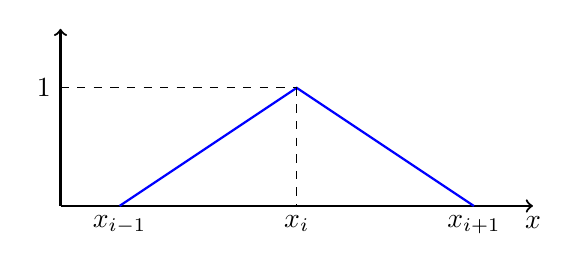
\begin{tikzpicture}[scale=1.5]
                    \draw[->, thick] (0,0) -- (4,0) node[anchor=north] {$x$};
                    \draw[->, thick] (0,0) -- (0,1.5);
                    \draw[thick, blue] (0.5,0) -- (2,1) -- (3.5,0);
                    \draw[dashed] (2,1) -- (2,0) node[anchor=north] {$x_i$};
                    \node[anchor=north] at (0.5,0) {$x_{i-1}$};
                    \node[anchor=north] at (3.5,0) {$x_{i+1}$};
                    \node[anchor=east] at (0,1) {$1$};
                    \draw[dashed] (0,1) -- (2,1);
                \end{tikzpicture}
            \end{center}

\end{frame}

\begin{frame}[t]{Piecewise Linear Approximation and Derivatives}
    A function $u_h \in \mathcal{P}^1_h$ is a linear combination of  hat functions: $u_h(x) = \sum_{i=1}^N u_i \phi_i(x)$.
    
    \begin{columns}
        \begin{column}{0.5\textwidth}
            \begin{center}
            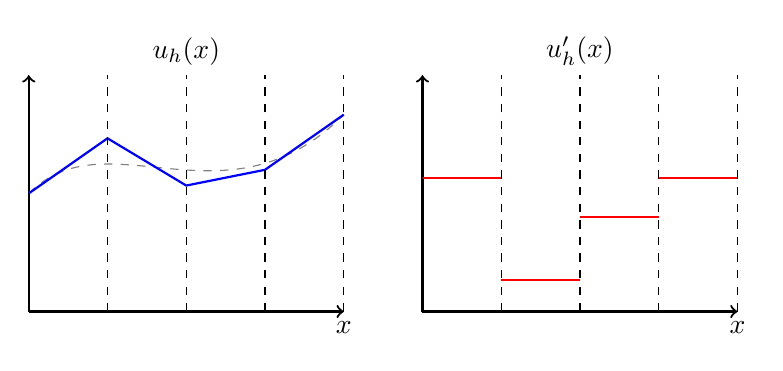
\begin{tikzpicture}[scale=1]
                \draw[->, thick] (0,-1) -- (4,-1) node[anchor=north] {$x$};
                \draw[->, thick] (0,-1) -- (0,2);
                \draw[gray, dashed] (0,0.5) .. controls (1,1.5) and (2.5,0) .. (4,1.5);
                \draw[thick, blue] (0,0.5) -- (1,1.2) -- (2,0.6) -- (3,0.8) -- (4,1.5);
                \foreach \x in {0,1,2,3,4} \draw[dashed] (\x,-1) -- (\x,2);
                \node[anchor=south] at (2,2) {$u_h(x)$};
                \only<1>{ 
                    \draw[->, thick] (5,-1) -- (9,-1) node[anchor=north] {$x$};
                    \draw[->, thick] (5,-1) -- (5,2);
                    \draw[thick, red] (5,0.7) -- (6,0.7);
                    \draw[thick, red] (6,-0.6) -- (7,-0.6);
                    \draw[thick, red] (7,0.2) -- (8,0.2);
                    \draw[thick, red] (8,0.7) -- (9,0.7);
                    \foreach \x in {5,6,7,8,9} \draw[dashed] (\x,-1) -- (\x,2);
                    \node[anchor=south] at (7,2) {$u_h'(x)$};
                }
            \end{tikzpicture}
            \end{center}
        \end{column}
        \begin{column}{0.5\textwidth}
            \only<2>{
                \textbf{The Need for Weak Forms:}
                \begin{itemize}
                    \item $u_h(x)$ is continuous ($C^0$).
                    \item $u_h'(x)$ is discontinuous
                    \item $u_h''(x)$ contains Dirac deltas at nodes 
                \end{itemize}
                \vspace{0.2cm}
                Therefore, $-\Delta u_h \notin L^2(\Omega)$. 
                \idea{Finite Elements (FE) work on \emph{weak} form}
                }
        \end{column}
    \end{columns}
\end{frame}

\section{The Finite Element (FE) Space}

\begin{frame}{Properties of the FE Space}
    Let $V_h = \text{span}\{\phi_1, \dots, \phi_N\}$ be our finite-dimensional approximation space.
    
    \vspace{0.3cm}
    \textbf{1. The Kronecker Delta Property:}
    By construction, 
    $$\phi_i(x_j) = \delta_{ij}.$$
    Therefore, 
$$ u_h(x_j) = \sum_i u_i \phi(x_j) = u_j \quad\Rightarrow\quad \text{Nodal values} $$
    
    \vspace{0.3cm}
    \textbf{2. The Interpolation Operator:}
For any continuous function $u \in C(\bar{\Omega})$, we define the Lagrange interpolant $\mathcal{I}_h: C(\bar{\Omega}) \to V_h$  as:
    $$ \mathcal{I}_h u(x) = \sum_{i=1}^N u(x_i) \phi_i(x) $$
    This guarantees that $\mathcal{I}_h u(x_j) = u(x_j)$ at all nodes.
\end{frame}

\section{Building the Linear System}

\begin{frame}{From Weak Form to Algebraic Equations}
    Consider the abstract discrete Galerkin problem: Find $u_h \in V_h$ such that
    $$ a(u_h, v_h) = \ell(v_h) \quad \forall v_h \in V_h $$
   .
    
    \vspace{0.3cm}
    \textbf{Step 1: Test against basis functions.}
    Since the equation holds for all $v_h \in V_h$, then $\forall v_h \in V_h \Leftrightarrow \forall \phi_i, i\in \{1,\dots, N\}$:
    $$ a(u_h, \phi_i) = \ell(\phi_i) \quad \forall i \in \{1, \dots, N\} $$
    
    \vspace{0.3cm}
    \textbf{Step 2: Expand the trial function.}
    We substitute the expansion $u_h = \sum_{j=1}^N u_j \phi_j$ into the bilinear form:
    $$ a\left(\sum_{j=1}^N u_j \phi_j, \phi_i\right) = \ell(\phi_i) \quad \forall i \in \{1, \dots, N\} $$
\end{frame}

\begin{frame}{The Stiffness Matrix and Load Vector}
    \textbf{Step 3: Extract the linear system.}
    Using the linearity of $a(\cdot, \phi_i)$:
    $$ \sum_{j=1}^N \underbrace{a(\phi_j, \phi_i)}_{K_{ij}}\underbrace{u_j}_{U_j} = \underbrace{\ell(\phi_i)}_{F_i} \quad \forall i \in \{1, \dots, N\} $$
    
    This is a matrix-vector system $K U = F$:
    \begin{itemize}
        \item $U = (U_1, \dots, U_N) \in \R^N$ unknown nodal values.
        \item $K_{ij} = a(\phi_j, \phi_i) \in \R^{N\times N}$ is the \textbf{Stiffness Matrix} (or system matrix).
        \item $F_i = \ell(\phi_i) \in \R^N$ is the \textbf{Load Vector} (or right-hand side).
    \end{itemize}
    
    \textit{Sparsity:} $\phi_j$ and $\phi_i$ have compact support, so $a(\phi_j, \phi_i) = 0$ unless nodes $i$ and $j$ share an element.
\end{frame}

\section{Example: The 1D ADR Problem}

\begin{frame}{The Advection-Diffusion-Reaction Equation}
    Let us approximate the ADR problem with a $\P_1$  FE space:
    $$ -\nu u'' + c u' + \sigma u = 1 \quad \text{in } (0, L), \quad u(0) = u(L) = 0 $$
    where $\nu > 0$ (diffusion), $c \in \mathbb{R}$ (advection), and $\sigma > 0$ (reaction) are constants.
    
    \vspace{0.3cm}
    \textbf{Weak Formulation:} Find $u \in H^1_0(\Omega)$ such that
    $$ \int_0^L \nu u' v' \, dx + \int_0^L c u' v \, dx + \int_0^L \sigma u v \, dx = \int_0^L v \, dx \quad \forall v \in H^1_0(\Omega) $$
    
    Here, our bilinear and linear forms are:
    \begin{align*}
        a(u, v) &= \nu(u', v') + c(u', v) + \sigma(u, v) \\
        \ell(v) &= (f, v)
    \end{align*}
\end{frame}

\begin{frame}{Analitic Assembly for ADR}
    The entries of the stiffness matrix $K_{ij} = a(\phi_j, \phi_i)$ are computed as:
    $$ K_{ij} = \nu \int_0^L \phi_j' \phi_i' \, dx + c \int_0^L \phi_j' \phi_i \, dx + \sigma \int_0^L \phi_j \phi_i \, dx $$
    
    Assume a uniform mesh with step size $h$. The basis functions $\phi_i$ only overlap with $\phi_{i-1}$, $\phi_i$, and $\phi_{i+1}$. 
    
    \begin{itemize}
        \item \textbf{Diffusion (Stiffness):} $\nu \int \phi_j' \phi_i' \rightarrow \frac{\nu}{h} [-1, 2, -1]$ \hfill (centered differences)
        \item \textbf{Advection:} $c \int \phi_j' \phi_i \rightarrow \frac{c}{2} [-1, 0, 1]$ \hfill (centered differences)
        \item \textbf{Reaction (Mass):} $\sigma \int \phi_j \phi_i \rightarrow \frac{\sigma h}{6} [1, 4, 1]$  \hfill (different!)
        \item \textbf{Load:} $F_i = \int_0^L \phi_i(x) \, dx = h$
    \end{itemize}
\end{frame}

\begin{frame}{ADR cont'd}
    \textbf{1. Diffusion Term (Stiffness):}
    \begin{itemize}
        \item $K_{ii} = \nu \int \phi_i' \phi_i' dx = \nu \left( \int_{x_{i-1}}^{x_i} \frac{1}{h^2} dx + \int_{x_i}^{x_{i+1}} \frac{1}{h^2} dx \right) = \nu \left( \frac{h}{h^2} + \frac{h}{h^2} \right) = \frac{2\nu}{h}$.
        \item $K_{i, i-1} = \nu \int_{x_{i-1}}^{x_i} \phi_{i-1}' \phi_i' dx = \nu \int_{x_{i-1}}^{x_i} (-\frac{1}{h})(\frac{1}{h}) dx = -\frac{\nu}{h}$.
    \end{itemize}

    \vspace{0.2cm}
    \textbf{2. Advection Term (Skew-Symmetric):}
    \begin{itemize}
        \item $K_{ii} = c \int \phi_i' \phi_i dx = c \left( \left[\frac{1}{2}\phi_i^2\right]_{x_{i-1}}^{x_i} + \left[\frac{1}{2}\phi_i^2\right]_{x_i}^{x_{i+1}} \right) = c(\frac{1}{2} - 0 + 0 - \frac{1}{2}) = 0$.
        \item $K_{i, i+1} = c \int_{x_i}^{x_{i+1}} \phi_{i+1}' \phi_i dx = c \int_{x_i}^{x_{i+1}} (\frac{1}{h})(\frac{x_{i+1}-x}{h}) dx = \frac{c}{h^2} \left[x_{i+1}x - \frac{x^2}{2}\right]_{x_i}^{x_{i+1}} = \frac{c}{2}$.
    \end{itemize}

    \vspace{0.2cm}
    \textbf{3. Reaction Term (Mass):}
    \begin{itemize}
        \item $K_{ii} = \sigma \int \phi_i^2 dx = \sigma \cdot 2 \int_0^h (\frac{x}{h})^2 dx = \frac{2\sigma}{h^2} \frac{h^3}{3} = \frac{2\sigma h}{3}$.
        \item $K_{i, i-1} = \sigma \int_{x_{i-1}}^{x_i} \phi_{i-1} \phi_i dx = \sigma \int_0^h (1-\frac{x}{h})(\frac{x}{h}) dx = \frac{\sigma}{h} [ \frac{x^2}{2} - \frac{x^3}{3h} ]_0^h = \frac{\sigma h}{6}$.
    \end{itemize}
\end{frame}

\begin{frame}\frametitle{ADR: Code}
    \idea{Console}
\end{frame}

\begin{frame}
    \titlepage
\end{frame}


\end{document}
